\section{Setup}
\label{sec:setup}

We aim to predict the task performance of LMs with an arbitrary \textit{training scale} -- the combination of model size ($N$) and number of training tokens ($D$).
As recent LMs are overtrained \citep{Dubey2024TheL3,Li2024DataCompLMIS,Bai2023QwenTR}, we do not constrain $N$ and $D$ to stay close to the compute-optimal regime \citep{Hoffmann2022TrainingCL}.
We validate our predictions on the \basemodelname{} models after stage 1 pretraining and before stage 2 annealing \citep{OLMo20242O2}; a 7B model trained to 4T tokens (``\textbf{7B-4T}'') and a 13B model trained to 5T tokens (``\textbf{13B-5T}''), both trained from scratch with the same data mixture.
These are \textit{target models}. 

\subsection{Ladder models}
\label{sec:ladder}

To predict the performance of large models, we extrapolate from data points collected from training many small models (``\textbf{ladder models}'').
These models have the same architecture and are trained with the same data mix as the target models. 
This is useful for guiding pretraining development, as data mixtures and modeling decisions can be tested in a controlled setting. 
The models span a relatively wide range of model size and training data size, while collectively costing a small fraction of compute used to train the target models.  

We define four model sizes $N \in $ \{ 190M, 370M, 760M, 1.3B \} (considering only non-embedding parameters) by varying the width and depth of the transformer.
% For each model size, we train it to different multiples of the ``Chinchilla optimal'' number of tokens.
We use $D = 20 \cdot N$ as the Chinchilla optimal setting \citep{Hoffmann2022TrainingCL} (denoted ``1xC''), and train each model with number of tokens $D \in $ \{ 1xC, 2xC, 5xC, 10xC \}.
In total, we train $4 \times 4 = 16$ models.
We save intermediate checkpoints every 200 steps for 1xC and 2xC runs, every 500 steps for 5xC runs, and every 1000 steps for 10xC runs.
\autoref{tab:hparams} lists the configurations of each model size.

\begin{table*}[t]
\small
\setlength{\tabcolsep}{3pt}
\centering
\caption{
    Model setup.
    Up to 1.3B are ladder models; 7B-4T and 13B-5T are target models.
}
\resizebox{0.9 \textwidth}{!}{%
\begin{tabular}{l | c c c c | c c}
\toprule
& \textbf{190M} & \textbf{370M} & \textbf{760M} & \textbf{1.3B} & \textbf{7B-4T} & \textbf{13B-5T} \\
\midrule
Model size ($N$) & 190,354,176 & 371,262,464 & 758,220,288 & 1,279,395,840 & 6,887,575,552 & 13,202,396,160 \\
1xC data size ($D$) & 3,807,083,520 & 7,425,249,280 & 15,164,405,760 & 25,587,916,800 & -- & -- \\
Batch size (sequences) & 128 & 192 & 320 & 384 & 1,024 & 2,048 \\
Batch size (tokens) & 524,288 & 786,432 & 1,310,720 & 1,572,864 & 4,194,304 & 8,388,608 \\
Training steps (1xC) & 7,272 & 9,452 & 11,580 & 16,279 & -- 
& -- \\
Peak LR & $9.7 \times 10^{-4}$ & $7.8 \times 10^{-4}$ & $6.1 \times 10^{-4}$ & $5.2 \times 10^{-4}$ & $3.0 \times 10^{-4}$ & $9.0 \times 10^{-4}$ \\
Warmup steps & 363 & 472 & 578 & 813 & 2000 & 1000 \\
\midrule
Dimension & 768 & 1,024 & 1,536 & 2,048 & 4,096 & 5,120 \\
Num heads & 12 & 16 & 16 & 16 & 32 & 40 \\
Num layers & 12 & 16 & 16 & 16 & 32 & 40 \\
MLP ratio & 8 & 8 & 8 & 8 & 5.375 & 4 \\
\bottomrule
\end{tabular}
}%
\label{tab:hparams}
\vspace{-12pt}
\end{table*}


The target models are trained with a cosine LR schedule with linear warmup, where the LR decays to 10\% of the peak LR over a horizon of 5T tokens.
We match this in the ladder models, where the decay horizon is adjusted to match the training data size of each model.
Unfortunately, the \basemodelname{} 7B model was only trained to 3.9T tokens in stage 1 pretraining, whereas the cosine scheduler was set to 5T tokens. 
%Prior work has shown that LR decay has a big impact on the performance of pretrained LMs.
To account for this incomplete training, we train this model with an additional 50B tokens where we linearly decay the LR down to 10\%.
Our target 7B-4T model is thus trained on a total of 3.95T tokens, where the linear decay instead of the slower cosine decay allows us to use fewer tokens.

For the ladder models, we set the peak LR, batch size, and warmup steps by extrapolating from the configuration of 7B-4T using the method introduced in \citet{Porian2024ResolvingDI}.
All other configurations follow from the 7B-4T model.

\tightparagraph{Compute cost.}
Using $C \approx 6 N D$ to estimate the compute \citep{Kaplan2020ScalingLF}, the total amount of compute used for training the ladder models is $5.2 \times 10^{21}$ FLOPs.
This is only \textbf{3.2\%} of that used for training the 7B-4T model ($1.6 \times 10^{23}$ FLOPs), \textbf{1.3\%} of the 13B-5T model ($3.9 \times 10^{23}$ FLOPs), and less than \textbf{1.0\%} of both target models combined.

\subsection{Intermediate features and accuracy}
\label{sec:task_setup}

%We focus on multiple-choice tasks.

\begin{table*}[t]
\small
\centering
\caption{
    Example for RC format from HellaSwag \citep{zellers-etal-2019-hellaswag}.
    Tokens on which task loss is computed are marked in \textcolor{darkgreen}{green}.
}
\resizebox{0.9 \textwidth}{!}{%
\begin{tabular}{p{85pt}p{345pt}}
\toprule
\textbf{Original problem} & \texttt{A woman is outside with a bucket and a dog. The dog is running around trying to avoid a bath. She \newline A. rinses the bucket off with soap and blow dry the dog’s head. \newline B. uses a hose to keep it from getting soapy. \newline C. gets the dog wet, then it runs away again. \newline D. gets into a bath tub with the dog. \newline Answer: C} \\
\midrule
\textbf{Task loss calculation} & \texttt{Question: A woman is outside with a bucket and a dog. The dog is running around trying to avoid a bath. She \newline Answer: \textcolor{darkgreen}{gets the dog wet, then it runs away again.}} \\
\bottomrule
\end{tabular}
}%
\label{tab:format}
\vspace{-8pt}
\end{table*}


\tightparagraph{Task loss.}
We define task loss as the negative log-likelihood of the correct answer sequence, divided by its length in bytes, also known as the bits-per-byte (bpb) metric.
\autoref{tab:format} shows the problem formatting for computing task loss on an example.
We use bpb instead of normalizing by number of tokens to reduce the impact of the tokenizer.\footnote{similar to ``normalized NLL per char'' \citep{Dubey2024TheL3}.} 

\tightparagraph{TaskCE.}
Task cross-entropy loss which accounts for incorrect answers (\S\ref{app:task_ce}).

\tightparagraph{LM loss.}
Standard language modeling loss on the C4-en validation set \citep{Raffel2019ExploringTL}.

%, like considering both correct and incorrect answers in the task loss, and using a general language modeling loss. We find that some tasks may benefit from these alternative choices, but task loss works best for predicting task accuracy on MMLU, which is the task we care most about.

\tightparagraph{Task accuracy.}
Ranked classification (RC) and multiple-choice (MC) are two different \textit{formats} to pose multiple-choice problems.)
In RC, the predicted answer is the one with the minimum task loss.
In MC, all the answer choices are included in the prompt, and the predicted answer is the answer code (e.g., A, B, C, etc.) with the smallest loss \citep{gu2024olmes}.
Here, we focus on the RC format.\footnote{RC reliably measures progress for models across a wide range of scales, whereas MC capability does not emerge until the model has several billion parameters.}

\tightparagraph{Evaluation.}
Following \citet{Gadre2024LanguageMS}, we compute the relative error for the task accuracy to evaluate the goodness of prediction, defined as
$$
\text{Relative Error} = \frac{|\text{prediction} - \text{actual}|}{\text{actual}} \times 100\%.
$$ 

\subsection{Task selection}

We include the following 8 tasks from the OLMES evaluation suite \citep{gu2024olmes}:
MMLU \citep{hendryckstest2021},
HellaSwag \citep{zellers-etal-2019-hellaswag},
ARC-Challenge \citep{Clark2018Think},
ARC-Easy \citep{Clark2018Think},
PIQA \citep{Bisk_Zellers_Le_bras_Gao_Choi_2020},
CommonsenseQA \citep{talmor-etal-2019-commonsenseqa},
Social IQa \citep{sap-etal-2019-social},
and OpenBookQA \citep{mihaylov-etal-2018-suit}.
We exclude BoolQ \citep{clark-etal-2019-boolq} and Winogrande \citep{Sakaguchi_Le_Bras_Bhagavatula_Choi_2020}, %as their performance does not scale monotonically on the ladder models.
as the task loss and accuracy are noisier for these tasks.
\S\ref{sec_variance_analysis} discusses task predictability further.
We use the test set where possible, and fall back to the validation set otherwise.
For all tasks, we use the 5-shot setting provided in OLMES.
\autoref{tab:stacked_pred} shows the task statistics.

\begin{figure*}[t]
\small
\setlength{\tabcolsep}{3pt}
\centering
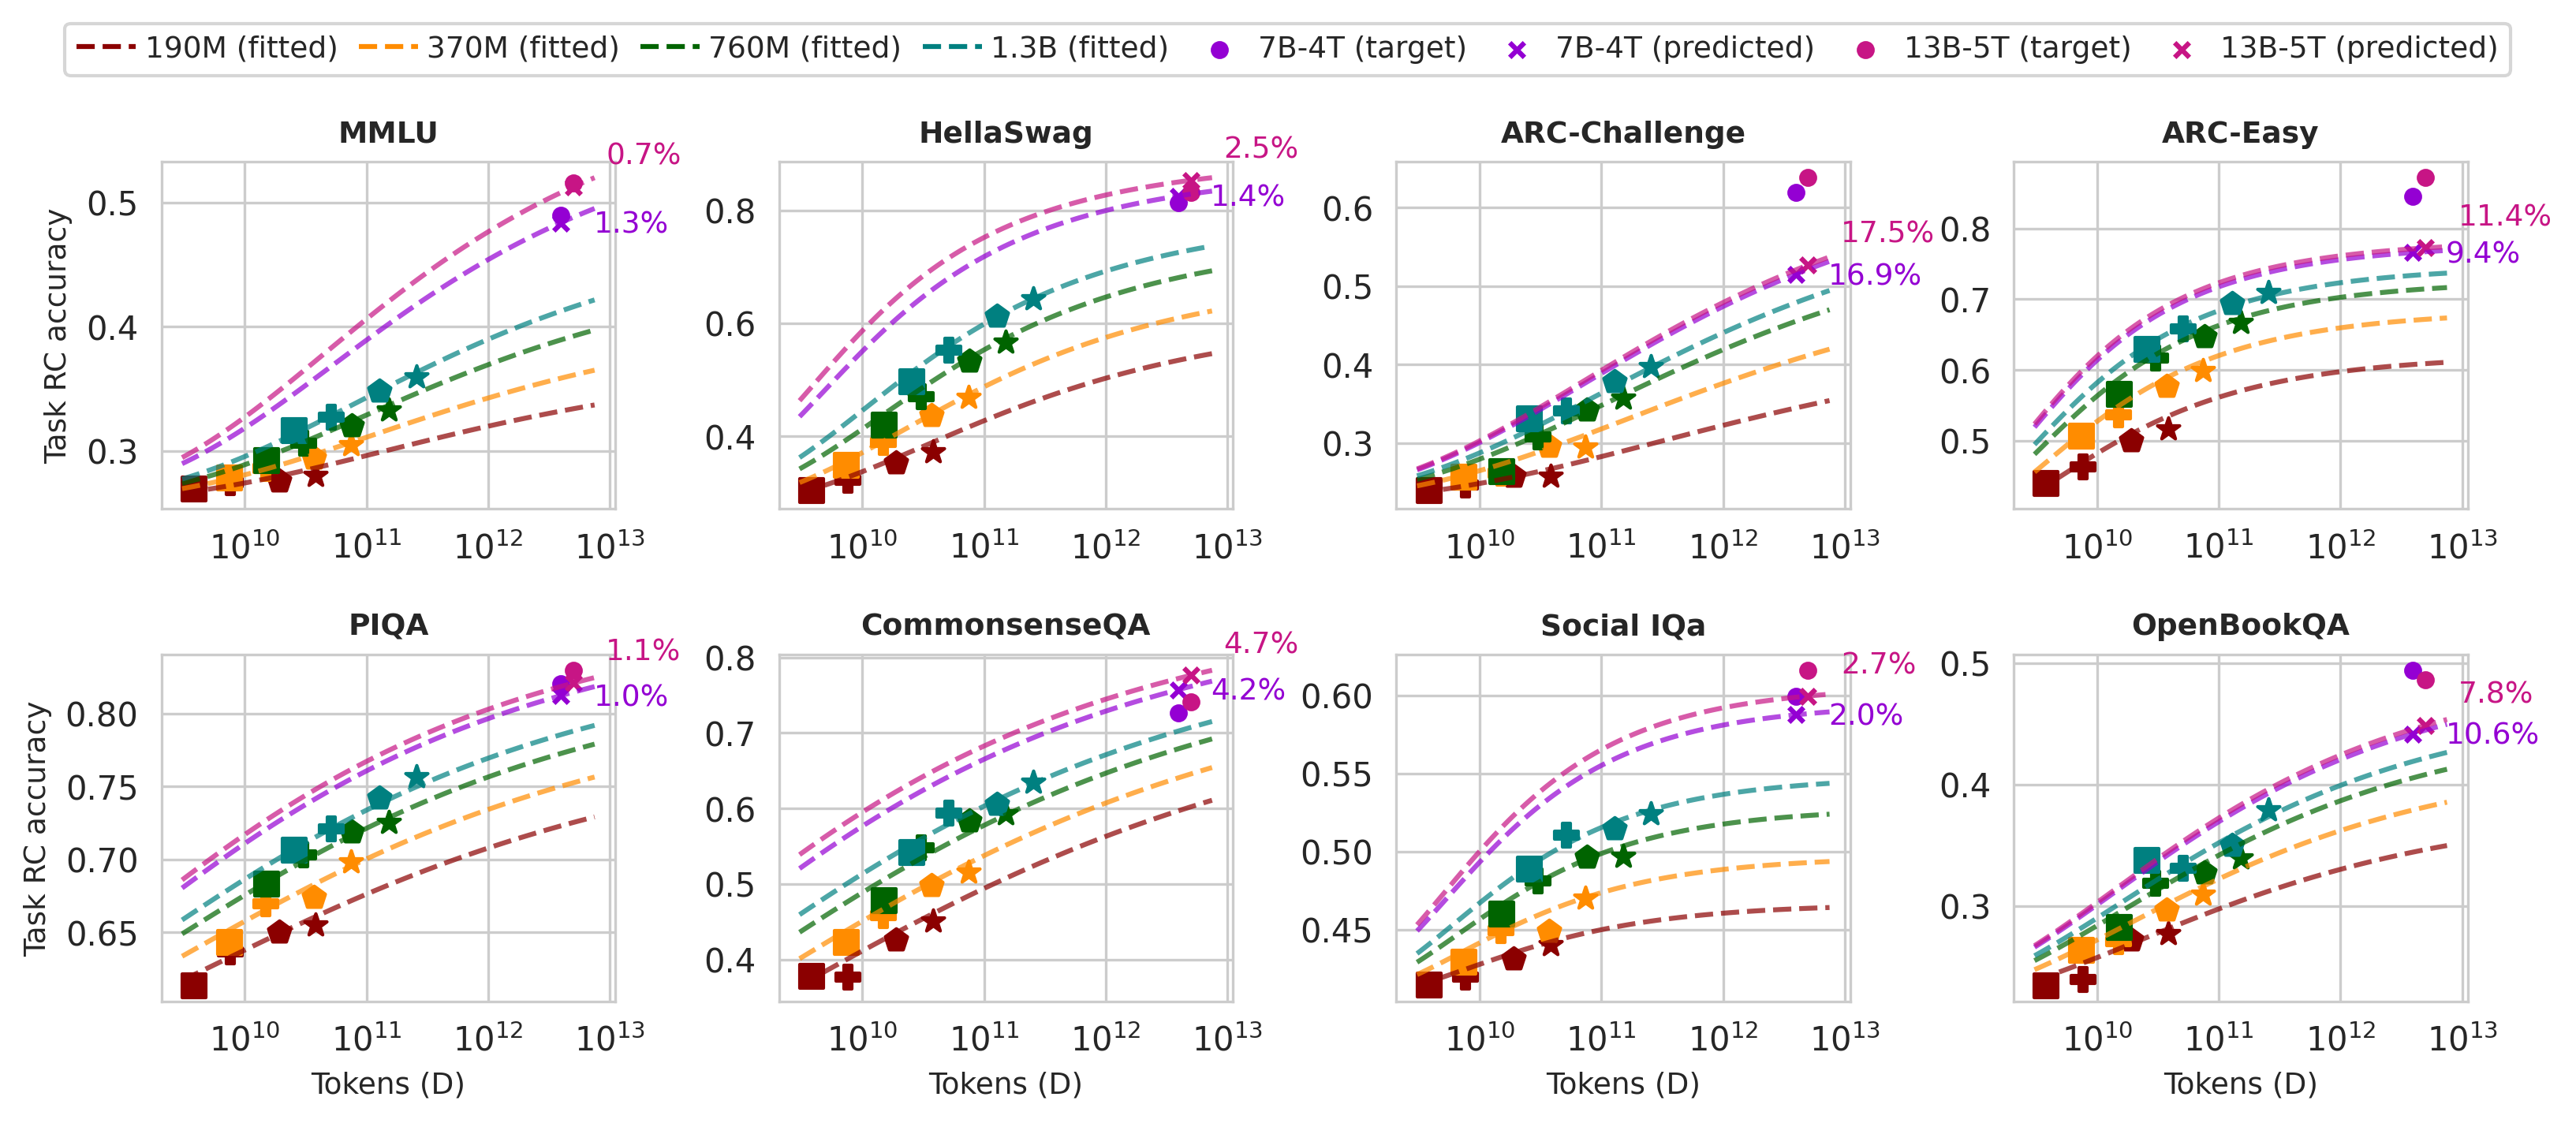
\includegraphics[scale=0.5]{images/chained_main.png}
\resizebox{0.75 \textwidth}{!}{%
\begin{tabular}{l c r | r r r r | r r r r}
\toprule
& & & \multicolumn{4}{c}{\textbf{7B-4T}} & \multicolumn{4}{c}{\textbf{13B-5T}}\\
\textbf{Task} & \textbf{Split} & \textbf{Examples} & Pred & Actual & Error & \%Error & Pred & Actual & Error & \%Error \\
\midrule
MMLU & test & 14,042 & 48.4 & 49.0 & 0.6 & 1.3\% & 51.3 & 51.6 & 0.3 & 0.7\% \\
HellaSwag & val & 10,042 & 82.5 & 81.3 & 1.2 & 1.4\% & 85.3 & 83.2 & 2.1 & 2.5\% \\
ARC-Challenge & test & 1,172 & 51.5 & 61.9 & 10.4 & 16.9\% & 52.7 & 63.8 & 11.1 & 17.5\% \\
ARC-Easy & test & 2,376 & 76.6 & 84.6 & 8.0 & 9.4\% & 77.2 & 87.2 & 10.0 & 11.4\% \\
PIQA & val & 1,838 & 81.2 & 82.0 & 0.8 & 1.0\% & 82.1 & 83.0 & 0.9 & 1.1\% \\
CommonsenseQA & val & 1,221 & 75.7 & 72.6 & 3.1 & 4.2\% & 77.6 & 74.1 & 3.5 & 4.7\% \\
Social IQa & val & 1,954 & 58.7 & 59.9 & 1.2 & 2.0\% & 59.9 & 61.6 & 1.7 & 2.7\% \\
OpenBookQA & test & 500 & 44.2 & 49.4 & 5.2 & 10.6\% & 44.9 & 48.6 & 3.7 & 7.8\% \\
\midrule
Average & -- & -- & -- & -- & 3.8 & 5.9\% & -- & -- & 4.2 & 6.1\% \\
\bottomrule
\end{tabular}
}%
\caption{
Task accuracy prediction for the target models using task loss as the intermediate feature.
\ding{110} = 1xC; \ding{58} = 2xC; $\pentagofill$ = 5xC; $\bigstar$ = 10xC.
Prediction error is next to the target.
}
\label{tab:stacked_pred}
\vspace{-8pt}
\end{figure*}


% \input{floats/tasks}

\section{Method}
\label{sec:method}

We break down task accuracy prediction into two steps: 1) predicting the intermediate feature (we use task loss to illustrate this), and 2) using it to predict the task accuracy.

%\S\ref{sec:ablations} discusses alternative choices for the intermediate feature. 

\subsection{Step 1: Use $(N, D)$ to predict the intermediate feature}
\label{sec:nd_to_loss}
% \akshita{i propose we make this step 1 to predict intermediate feature, and show bpb as an example (can explain this at the start of Method section). and we rewrite / remove the results preview and just say that other feature results are shown later ("Results preview" and reporting average error for all tasks currently makes it sound like bpb is the main, best method, which we want to avoid). rather than average, we can discuss individual tasks. this way, we don't commit to a flawed bpb based method, we just show it as one of the alternatives, and we expect different features to be used for different tasks. then, after variance analysis, which includes c4 and taskCE, we give recs - pick the intermediate feature with the lowest variance (i'm hoping this will align with our ablations table results)}

We consider three intermediate features: task loss, taskCE loss, and LM loss (defined in \S\ref{sec:setup}).

As proposed by \citet{Hoffmann2022TrainingCL} and followed by others \citep{Muennighoff2023ScalingDL,Gadre2024LanguageMS,Zhang2024MAPNeoHC}, the LM loss of a model on a held-out eval set can be modeled as a power function with respect to $N$ and $D$:
\begin{align}
L(N, D) &= A / N^\alpha + B / D^\beta + E,
\label{eqn:power}
\end{align}
where $A, B, \alpha, \beta, E$ are parameters to fit.

We postulate that \textbf{the same functional form applies to these losses}.
We validate this assumption by looking at the goodness of function fitting.

\tightparagraph{Function fitting.}
We take the loss value of the final checkpoint of each ladder model $\{ (N_i, D_i, L_i) \}_{i=1}^{n}$ (where $n = 16$), and use this data to fit the parameters of \autoref{eqn:power}.
We fit a separate set of parameters for each task.
Following \citet{Hoffmann2022TrainingCL},
we minimize the Huber loss between the logarithm of predicted and actual loss: $\frac{1}{n} \sum_{i=1}^{n} \text{Huber}_\delta \big( \log \hat{L}(N_i, D_i) - \log L_i \big)$, where $\delta = 10^{-3}$.
We optimize $A$ and $B$ in log space -- we apply transformation $a = \log A, b = \log B$ and optimize $(a, b, \alpha, \beta, E)$.
We use the L-BFGS-B optimizer as implemented in \texttt{scipy.minimize()}, with constraints $A, B, \alpha, \beta, E \geq 0$; with these constraints, the function is convex, and thus L-BFGS-B is guaranteed to converge.\footnote{To test if this function is convex, we confirm that the Hessian matrix of second derivatives is positive semi-definite everywhere.} 

We take the average loss over the last 5 checkpoints of each ladder model to reduce noise. 

\begin{figure*}[t]
\centering
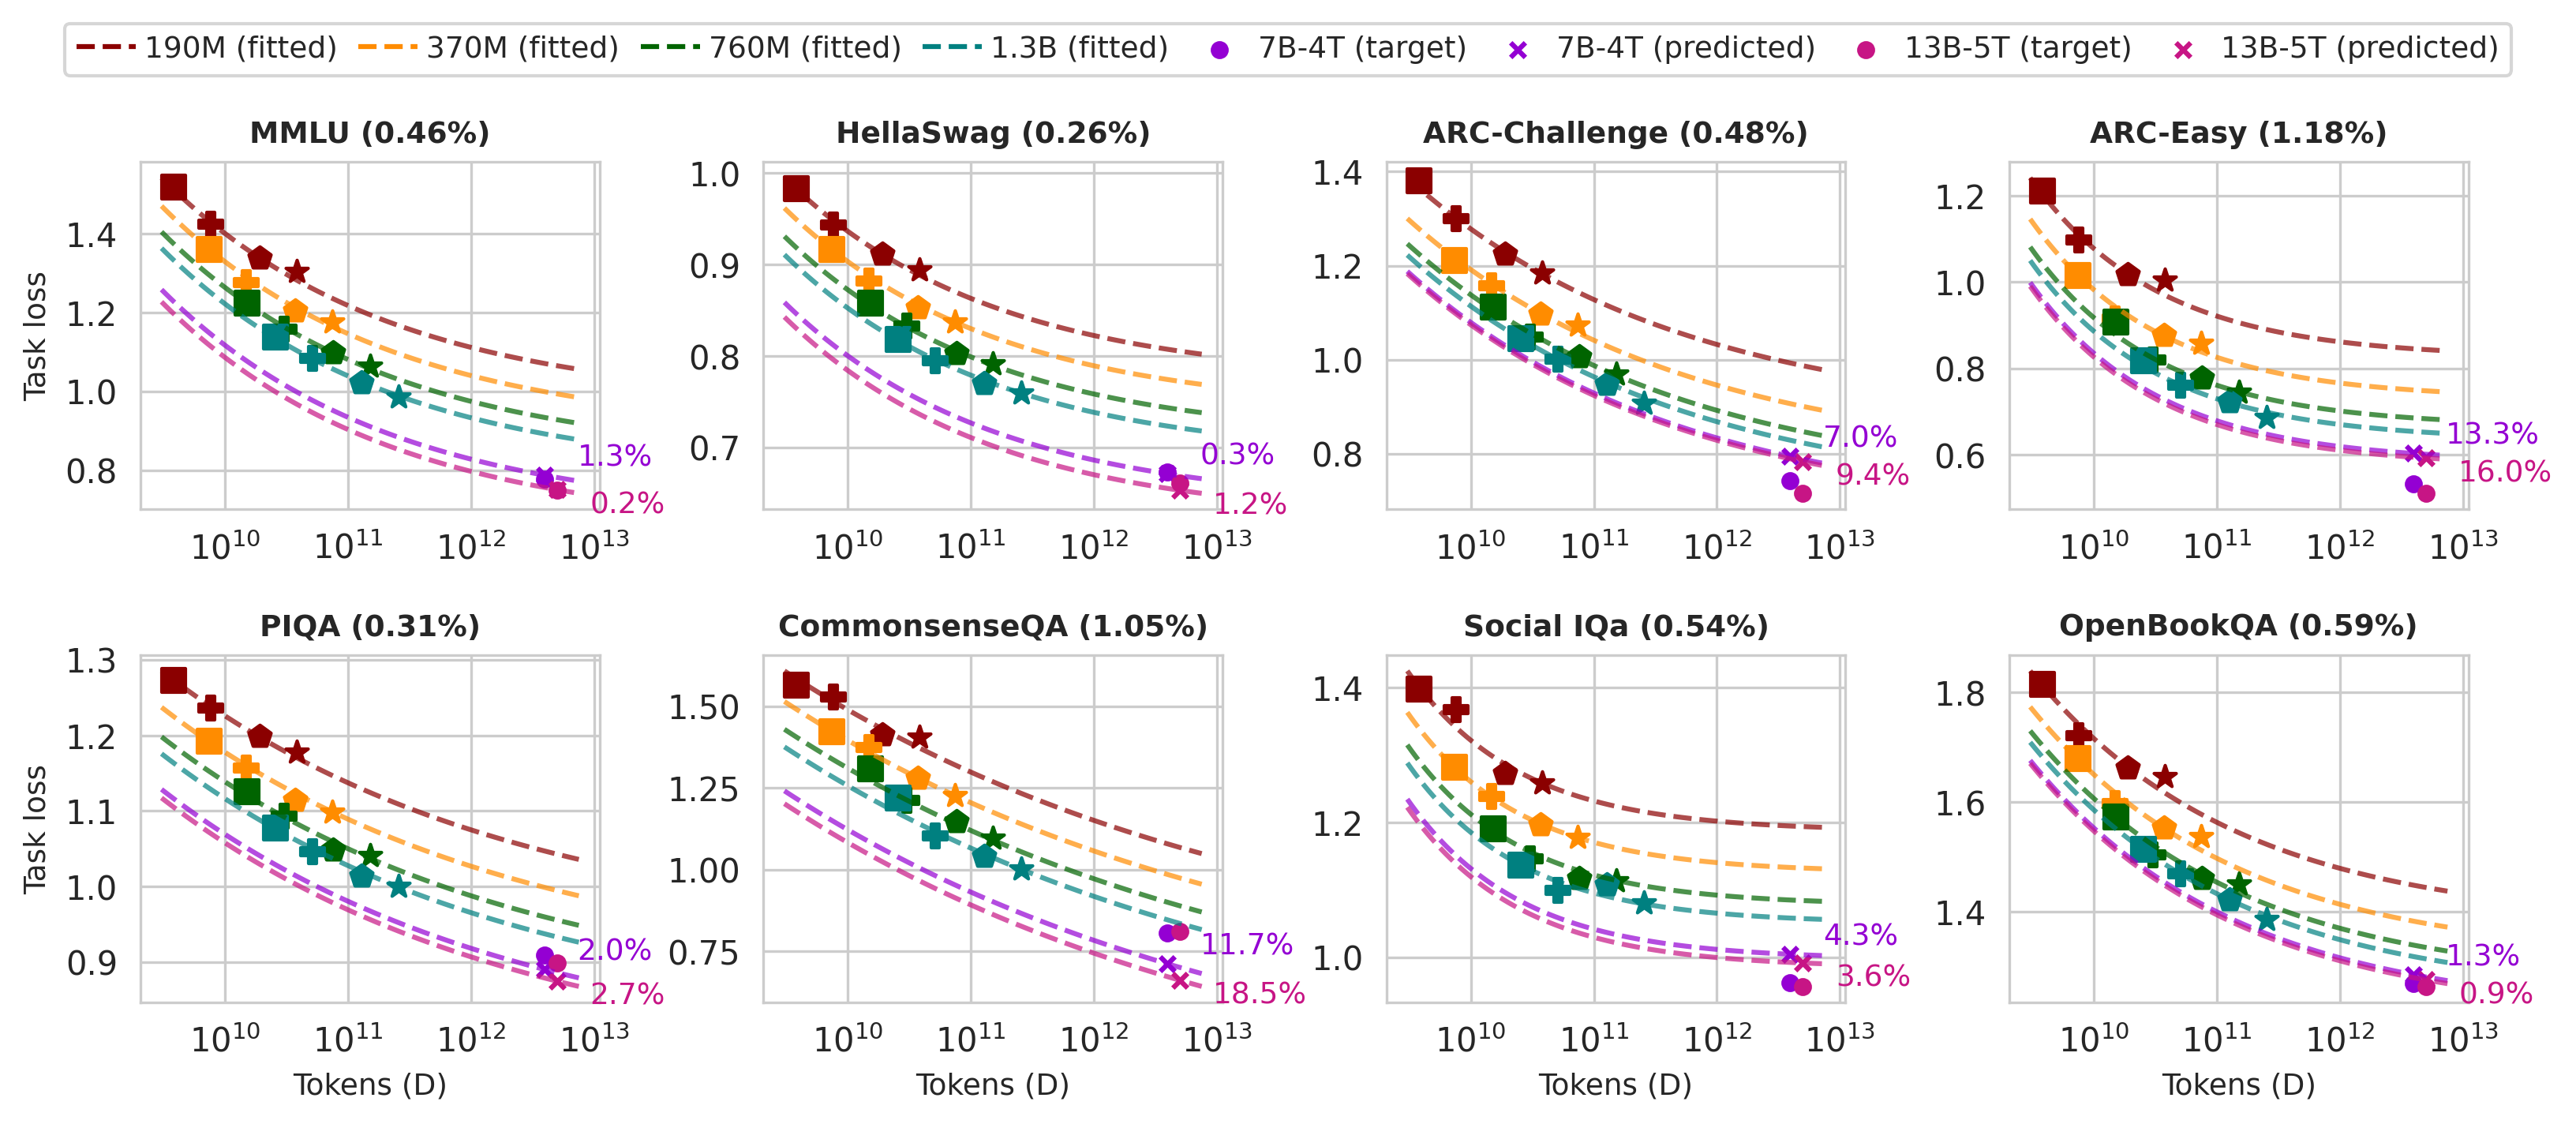
\includegraphics[width=\linewidth]{images/step1_main.png}
\vspace{-16pt}
\caption{
    Task loss vs training scale $(N, D)$, with fitting on the power function in \autoref{eqn:power}.
    \ding{110} = 1xC; \ding{58} = 2xC; $\pentagofill$ = 5xC; $\bigstar$ = 10xC.
    We report the average relative fitting error in parentheses after the task name, and prediction error next to the target model point.
    %In general, the power function fits well to data points from the ladder models, and the fitted function makes rather reliable predictions for the targer models.
    %See \autoref{tab:fitted_params} for the parameters of the fitted functions.
}
\label{fig:step1}
\vspace{-8pt}
\end{figure*}

\tightparagraph{Results preview.}
\autoref{fig:step1} shows the function fitting of step 1 on the ladder models, and the prediction of task loss as the intermediate feature for the target models. The power function gives an average relative \textit{fitting error} ranging from 0.2\% to 1.2\%, which suggests that \autoref{eqn:power} is a good functional form to describe task losses.
We have a relative \textit{prediction error} within 3\% on MMLU, HellaSwag, PIQA, and OpenBookQA.
The method underestimates the loss for CSQA, and overestimates on ARC-Challenge, ARC-Easy, and Social IQa.
On target models, across all tasks we get an average relative error of 5.2\% for 7B-4T, and 6.6\% for 13B-5T.
Results for the other intermediate features are discussed in \S\ref{app:task_ce} and \S\ref{app:c4}.

In \S\ref{app:flops_as_feature}, we use compute-FLOPs as input variable instead of $(N, D)$, and observe higher fitting errors for all tasks. We also note that FLOPs cannot distinguish between compute-optimal and overtrained models.
%, and ablate the design choices of step 1 in \S\ref{sec:ablations}.

% \subsection{Step 1: Use $(N, D)$ to predict task loss}
% \label{sec:nd_to_loss}
% \akshita{i propose we make this step 1 to predict intermediate feature, and show bpb as an example (can explain this at the start of Method section). and we rewrite / remove the results preview and just say that other feature results are shown later ("Results preview" and reporting average error for all tasks currently makes it sound like bpb is the main, best method, which we want to avoid). rather than average, we can discuss individual tasks. this way, we don't commit to a flawed bpb based method, we just show it as one of the alternatives, and we expect different features to be used for different tasks. then, after variance analysis, which includes c4 and taskCE, we give recs - pick the intermediate feature with the lowest variance (i'm hoping this will align with our ablations table results)}

% As proposed by \citet{Hoffmann2022TrainingCL} and followed by others \citep{Muennighoff2023ScalingDL,Gadre2024LanguageMS,Zhang2024MAPNeoHC}, the LM loss of a model on a held-out eval set can be modeled as a power function with respect to $N$ and $D$:
% \begin{align}
% L(N, D) &= A / N^\alpha + B / D^\beta + E,
% \label{eqn:power}
% \end{align}
% where $A, B, \alpha, \beta, E$ are parameters to fit.

% We postulate that \textbf{the same functional form applies to the task loss}.
% We validate this assumption by looking at the goodness of function fitting.

% \tightparagraph{Function fitting.}
% We take the loss value of the final checkpoint of each ladder model $\{ (N_i, D_i, L_i) \}_{i=1}^{n}$ (where $n = 16$), and use this data to fit the parameters of \autoref{eqn:power}.
% We fit a separate set of parameters for each task.
% Following \citet{Hoffmann2022TrainingCL},
% we minimize the Huber loss between the logarithm of predicted and actual loss: $\frac{1}{n} \sum_{i=1}^{n} \text{Huber}_\delta \big( \log \hat{L}(N_i, D_i) - \log L_i \big)$, where $\delta = 10^{-3}$.
% We optimize $A$ and $B$ in log space -- we apply transformation $a = \log A, b = \log B$ and optimize $(a, b, \alpha, \beta, E)$.
% We use the L-BFGS-B optimizer as implemented in \texttt{scipy.minimize()}, with constraints $A, B, \alpha, \beta, E \geq 0$; with these constraints, the function is convex, and thus L-BFGS-B is guaranteed to converge.\footnote{To test if this function is convex, we confirm that the Hessian matrix of second derivatives is positive semi-definite everywhere.} 

% We take the average task loss over the last 5 checkpoints of each ladder model to reduce noise. 

% \begin{figure*}[t]
\centering
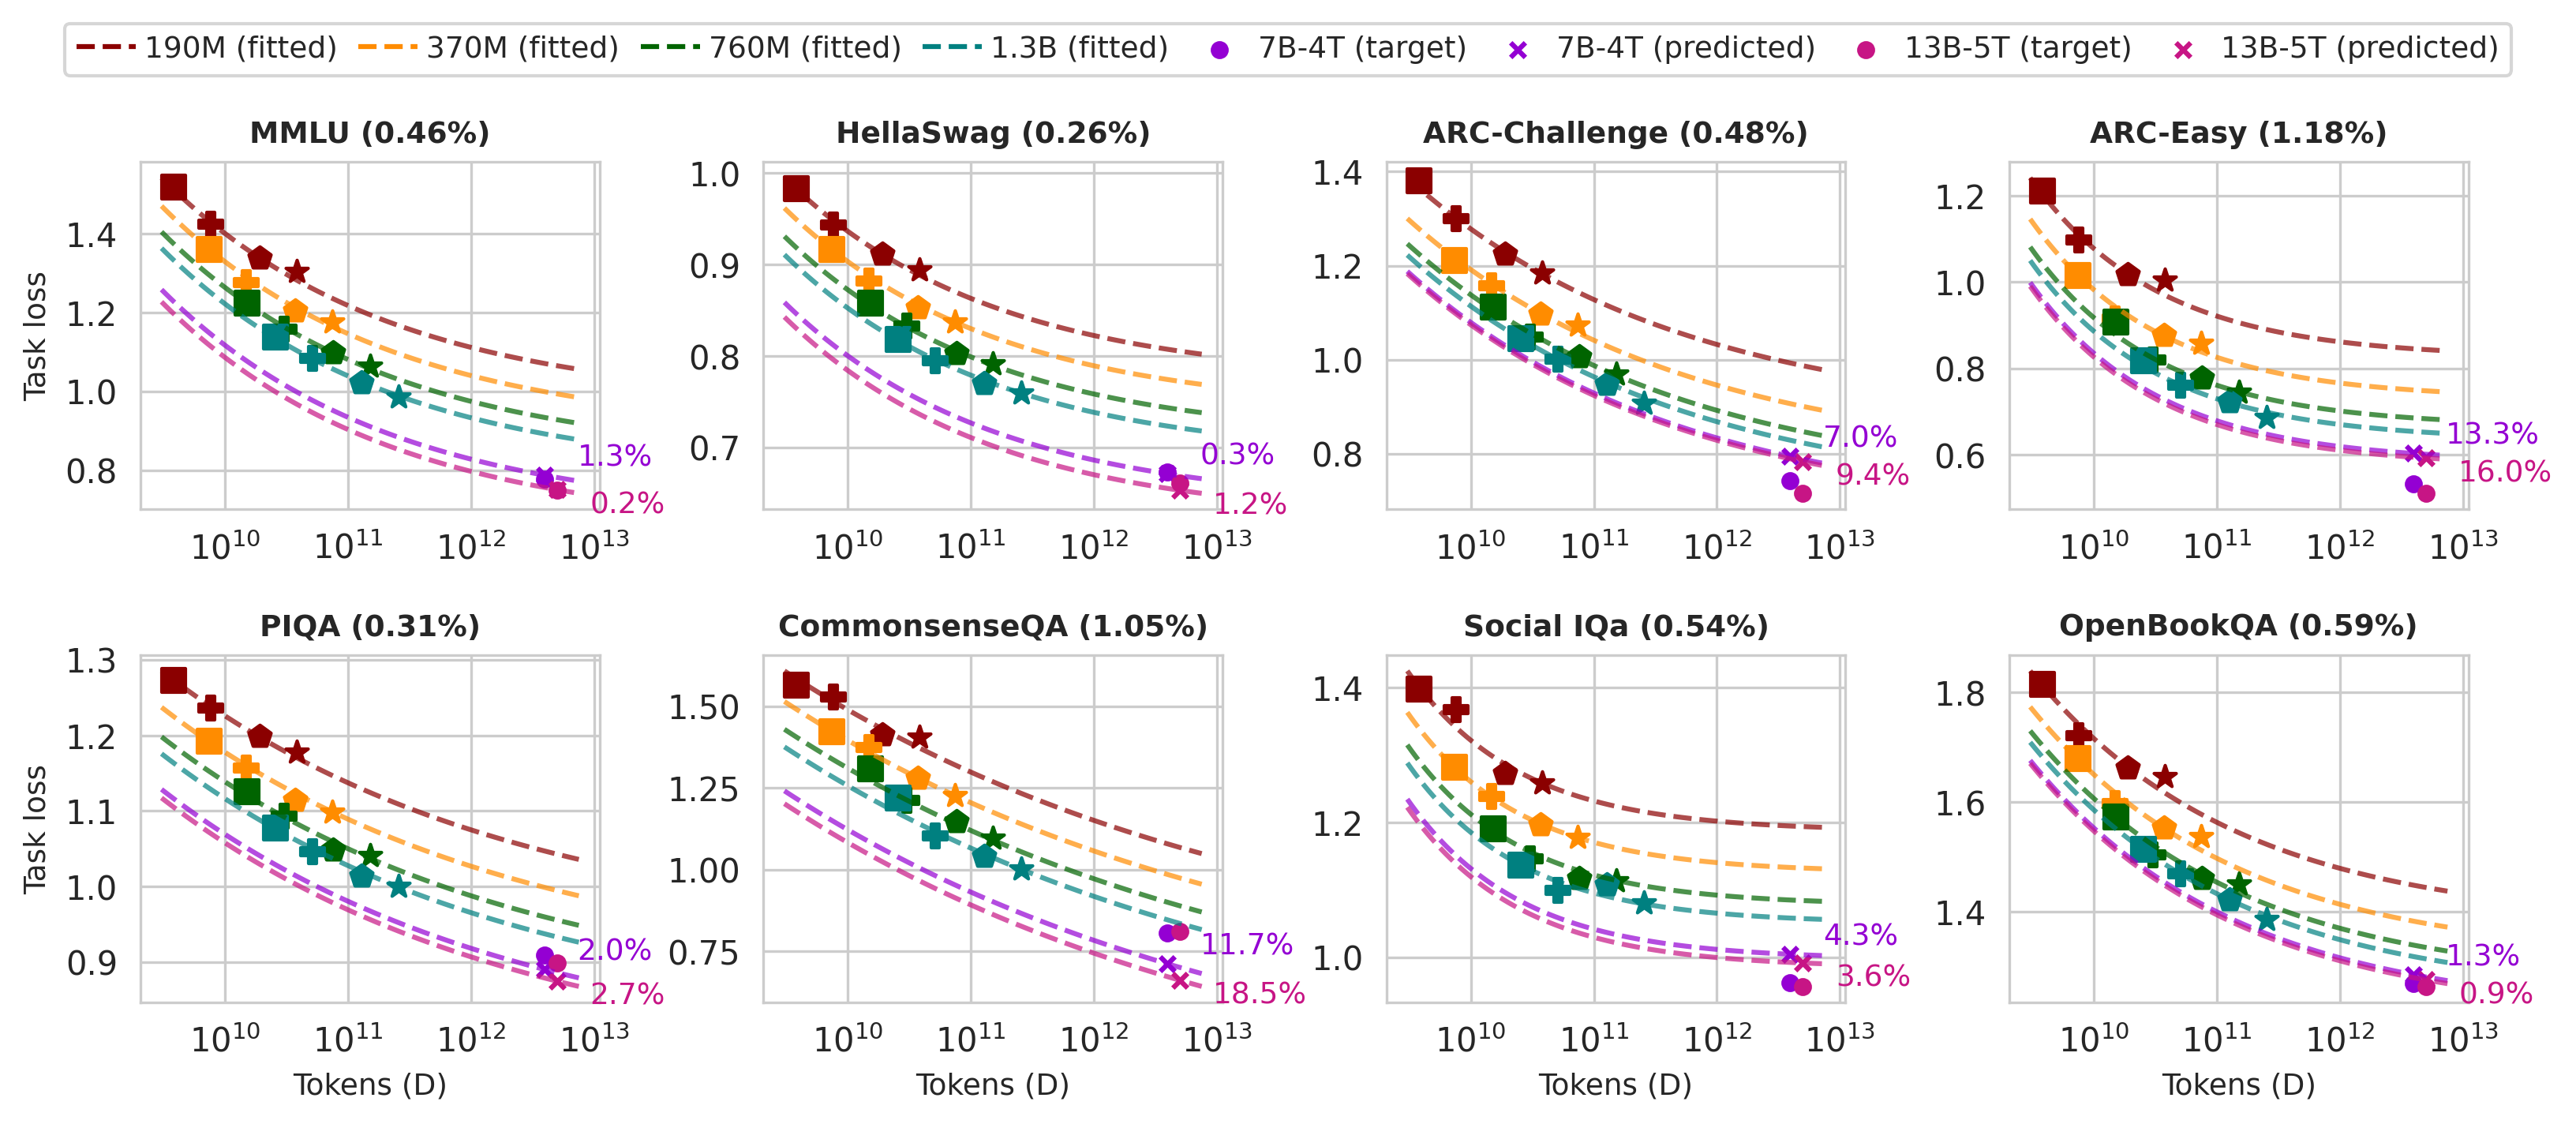
\includegraphics[width=\linewidth]{images/step1_main.png}
\vspace{-16pt}
\caption{
    Task loss vs training scale $(N, D)$, with fitting on the power function in \autoref{eqn:power}.
    \ding{110} = 1xC; \ding{58} = 2xC; $\pentagofill$ = 5xC; $\bigstar$ = 10xC.
    We report the average relative fitting error in parentheses after the task name, and prediction error next to the target model point.
    %In general, the power function fits well to data points from the ladder models, and the fitted function makes rather reliable predictions for the targer models.
    %See \autoref{tab:fitted_params} for the parameters of the fitted functions.
}
\label{fig:step1}
\vspace{-8pt}
\end{figure*}

% \tightparagraph{Results preview.}
% The power function fits the ladder models well, with relative fitting error ranging from 0.2\% to 1.2\% on all tasks.
% On target models, across all tasks we get an average relative error of 5.2\% for 7B-4T, and 6.6\% for 13B-5T.
% We present results on individual tasks in \S\ref{sec:results}. In \S\ref{app:flops_as_feature}, we use compute-FLOPs as input variable instead of $(N, D)$, and observe higher fitting errors for all tasks.
% %, and ablate the design choices of step 1 in \S\ref{sec:ablations}.

\subsection{Step 2: Use intermediate feature to predict accuracy}
\label{sec:loss_to_acc}

\begin{figure*}[t]
\centering
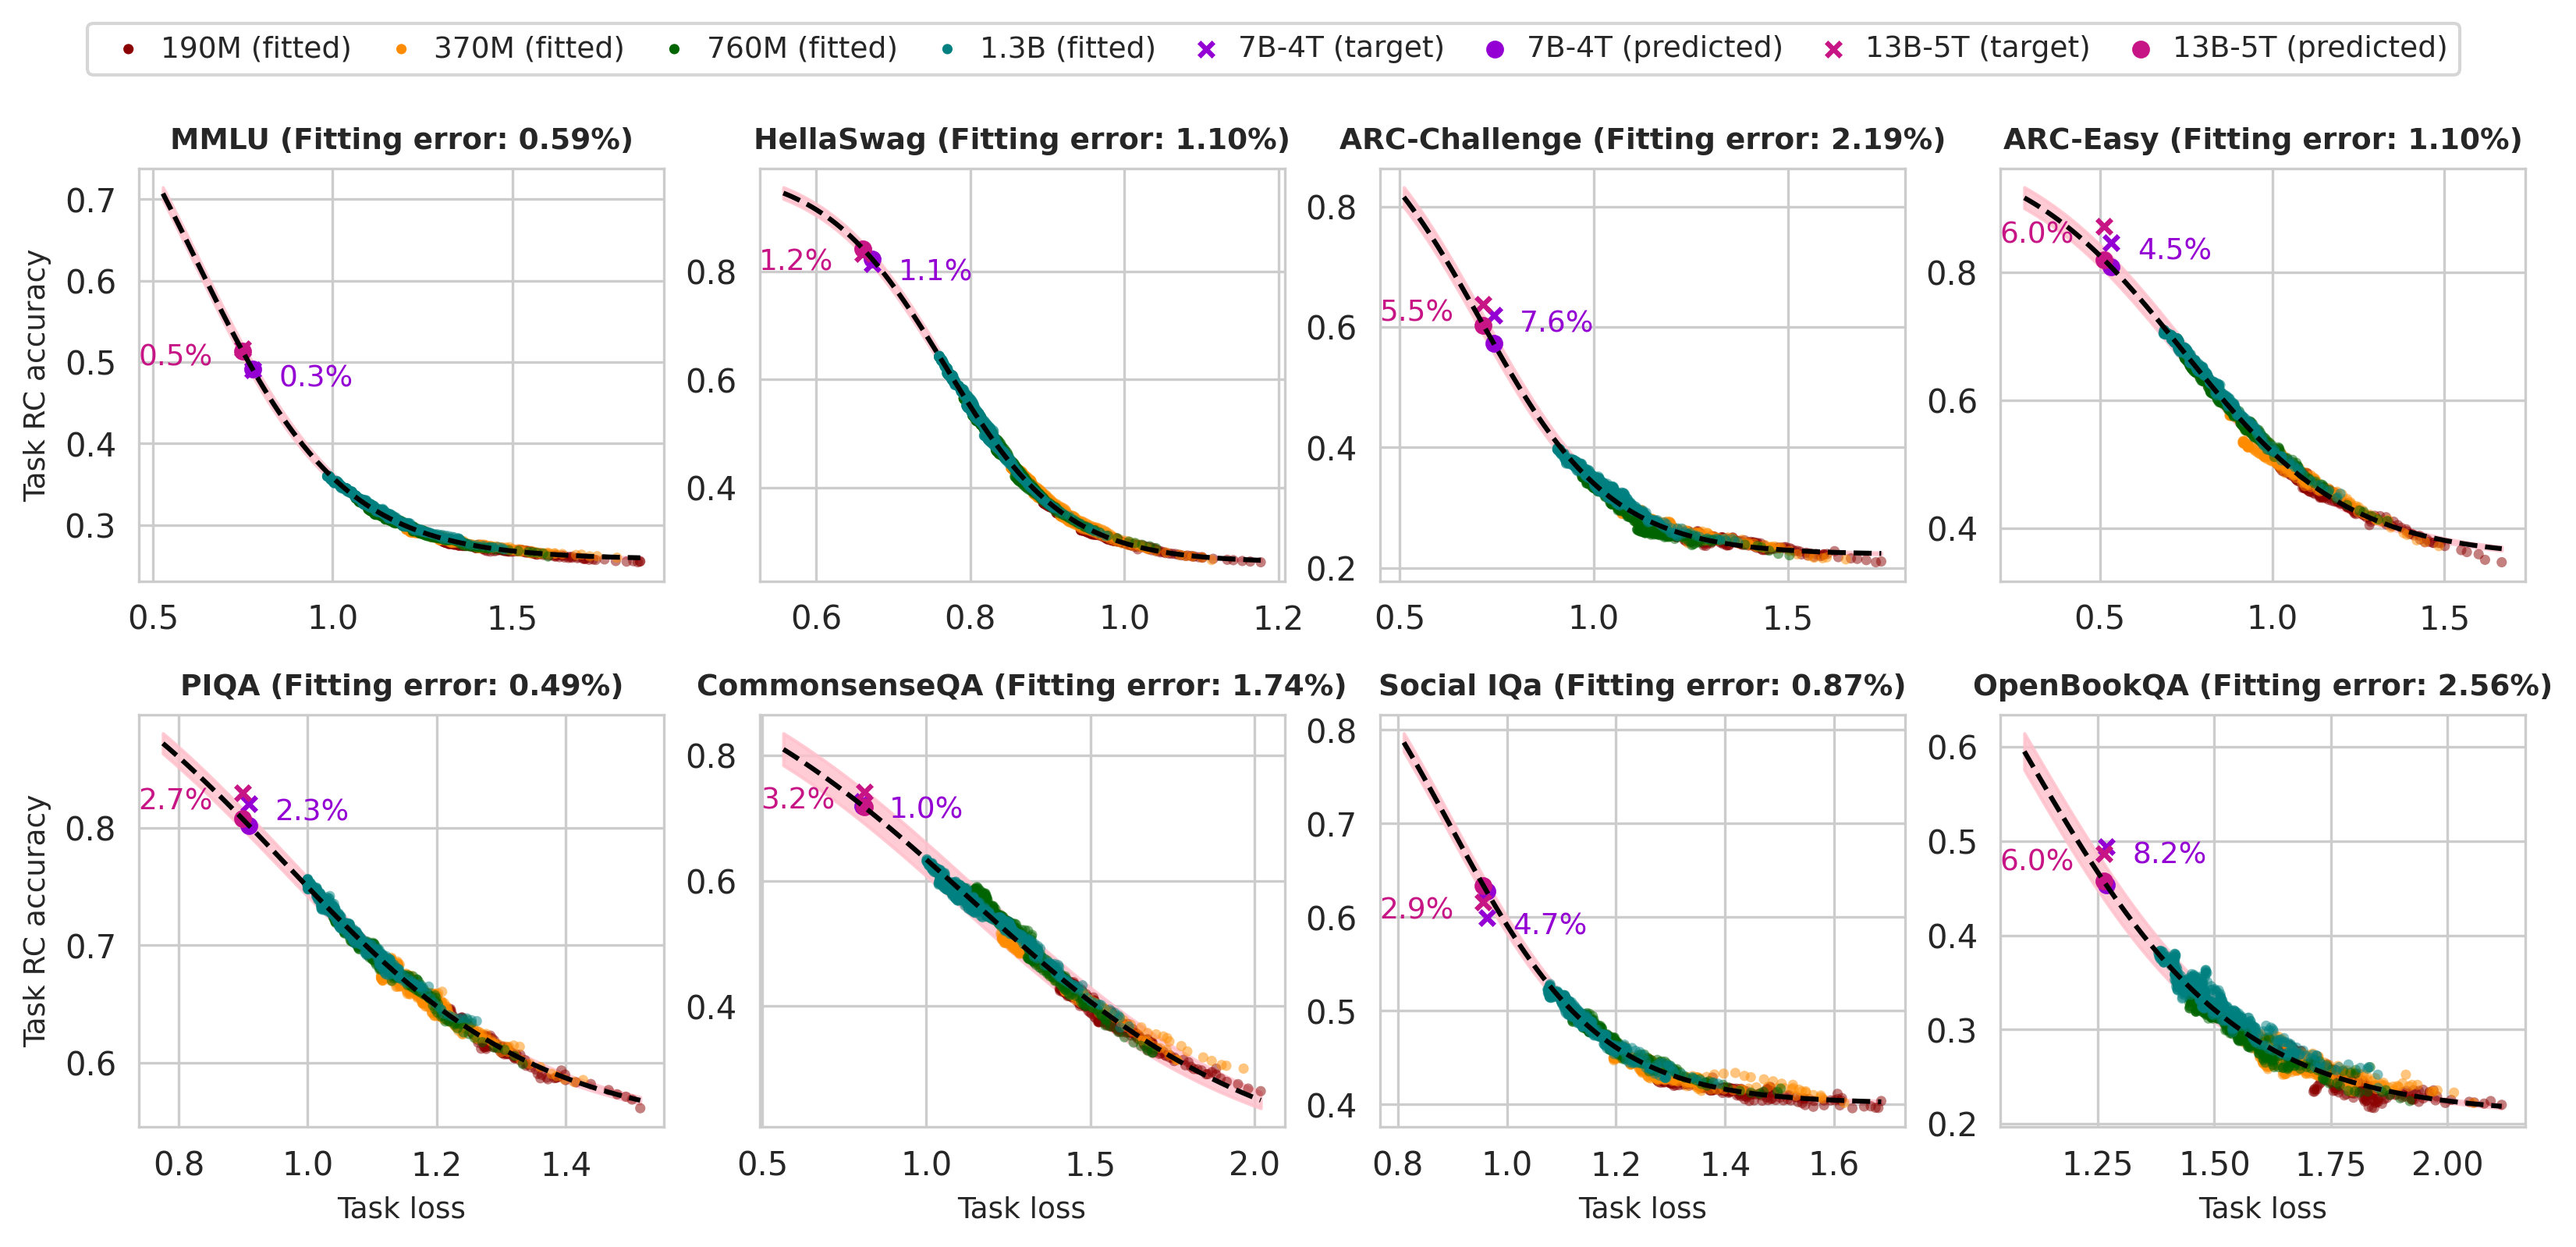
\includegraphics[width=\linewidth]{images/step2_main.png}
\vspace{-16pt}
\caption{
    Task RC accuracy vs task loss, with fitting on the sigmoid function in \autoref{eqn:sigmoid}.
    The prediction error is next to the target model point.
    %For each task, the data points collected from ladder models lie on a shared sigmoidal curve, and the fitted function makes rather reliable predictions for the target models. 
    The shaded area represents the prediction intervals for the fitted function.
    %See \autoref{tab:fitted_params} for the parameters of the fitted functions.
}
\label{fig:step2}
\vspace{-8pt}
\end{figure*}

Following \citet{Dubey2024TheL3}, we model the mapping from the intermediate loss to accuracy with a sigmoidal function:
\begin{equation}
    Acc(L) = \frac{a}{1 + e^{-k(L-L_0)}} + b
\label{eqn:sigmoid}
\end{equation}
where $a, b, k, L_0$ are parameters to fit.

The choice of a sigmoidal functional form is motivated as follows: a weak model has high task loss and random task accuracy, and a strong model has low task loss and high task accuracy that saturates at 100\%.
We observe (as shown in \autoref{fig:step2}) that the $(L_i, Acc_i)$ points collected from different ladder models tend to fall on a shared sigmoidal curve; this applies to both intermediate and final model checkpoints. 

\tightparagraph{Function fitting.}
We use the intermediate loss and accuracy values from both final and intermediate checkpoints of the ladder models $\{ (L_i, Acc_i) \}_{i=1}^m$ (where $m \approx 1400$) to fit the parameters of \autoref{eqn:sigmoid}.
We fit a separate set of parameters for each downstream task.
We minimize the L2 loss between the predicted and actual accuracy: $\frac{1}{m} \sum_{i=1}^{m}(\hat{Acc}(L_i) - Acc_i)^2$.
We use non-linear least squares implemented by \texttt{scipy.optimize.curve\_fit()} to fit this equation, as sigmoid functions are not convex. 

The variation from checkpoint to checkpoint can be high. To smoothen the noise, we apply a moving average on the intermediate loss and task accuracy over all checkpoints of each training run, with a window size of 5. We also discard the checkpoints from the first 10\% of each training run as these are quite noisy, and add an extra data point $(L=0.0, Acc=1.0)$ to the training pairs. This helps avoid the cases when the fitting function degenerates for very noisy data, and the ladder models are too small to do well on certain tasks.

\tightparagraph{Results preview.}

\autoref{fig:step2} shows the function fitting of step 2 on the ladder models, and the prediction of task accuracy for the target models using their \textit{actual} task loss as the intermediate feature.
For all tasks, all data points fit well with a shared sigmoidal function, with the average relative \textit{fitting error} ranging from 0.4\% to 2.6\%.
We get within 3\% relative \textit{prediction error} on MMLU, HellaSwag, PIQA, and CommonsenseQA.
%We overestimate Social IQa (+4.7\%, +2.9\%), and underestimate ARC-Challenge (-7.6\%, -5.5\%), ARC-Easy (-4.5\%, -6.0\%), and OpenBookQA (-8.2\%, -6.0\%).
%The underestimations happen when we cannot accurately extrapolate the slope of the sigmoidal function from data points collected from the small ladder models.
Overall, we get an average relative error of 3.7\% for 7B-4T, and 3.5\% for 13B-5T.
%, and ablate the design choices of step 1 in \S\ref{sec:ablations}.

\subsection{Chaining the two steps}
\label{sec:nd_to_acc}

We chain the two steps by first predicting the intermediate loss with the fitted function in step 1, and then inserting it into the fitted function in step 2 to predict the task accuracy.

\tightparagraph{Results preview.} 
Using task loss as the intermediate feature, we get an average absolute error of 3.8 points for 7B-4T, and 4.2 points for 13B-5T.
%We present results on individual tasks in \S\ref{sec:results}. 
In \S\ref{app:single_step}, we also show the results of predicting the task accuracy directly from (N, D) in a single step, and observe higher average prediction errors for both target models ($>$ 30 points). 
